\section{Question 3}\label{sec:q3}    

\textit{We consider a movement of a satellite around the Earth. From observation data can be concluded that the orbit of the satellite has a period of $T = 1.85$ hours, and that at a given time $t_0$ the radial and normal components of the satellite's velocity are given by $\dot{r} = -0.2481$ km/s and $r\dot{theta} = 6.5726$ km/s. Furthermore, it is known that the satellite is in a low eccentric orbit ($e < 0.3$).}

\subsection{3a}
\textit{From the general equation for an elliptical orbit, derive the following expressions for the radial and normal velocity components:} 
\begin{equation}
    \dot{r}=\dfrac {\mu }{H}e\sin \left( \theta \right) \quad ; \quad r\dot{\theta} =\dfrac {\mu }{H}\left( 1-e\cos \left( \theta \right) \right) 
\end{equation} \\

For a generic elliptic orbit, its radius is described by:
\begin{equation} \label{eq:elliptic}
    r = \frac{p}{1+e \cos(\theta)}
\end{equation}

\begin{figure}[H]
    \centering
    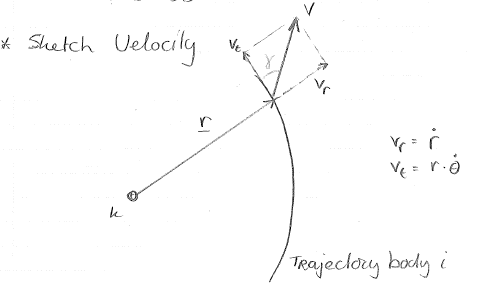
\includegraphics[width=0.5\columnwidth]{Figures/3a.png}
    \caption{Velocities of a body in orbit.}
    \label{fig:3a}
\end{figure}

The radial velocity as defined in figure \ref{fig:3a} equals:
\begin{equation}
    \dot{r}=V\cdot \sin \left( \gamma \right) \quad and so \quad V=\dfrac {\dot{r}}{\sin \left( \gamma \right) }
\end{equation}

For the tangential velocity, we have:
\begin{equation}
    r \cdot \dot{\theta}=V\cdot \cos \left( \gamma \right) \quad and so \quad V=\dfrac {r \dot{\theta}}{\cos \left( \gamma \right) } \\
\end{equation}

So the flight path angle can be defined as:
\begin{equation}
    \tan (\gamma) = \frac{\dot{r}}{r\dot{\theta}}
\end{equation}

Furthermore, for the angular momentum we can find:
\begin{equation}
\begin{split}
    H=rV_{t}=r\cdot r\cdot \dot{\theta} =r^{2}\dot{\theta} =v\cdot r\cdot \cos \left( \gamma \right)\\
    r\cdot \theta =\dfrac {H}{r} =\dfrac {H}{p}\left[ 1+e\cos \left( \theta \right) \right] \\
\end{split}
\end{equation}

Given the definition of the semi-latus rectum, namely that $p = H^2/\mu$, we can rewrite this further:
\begin{equation}
     r\cdot \theta =\dfrac {\mu}{H}\left[ 1+e\cos \left( \theta \right) \right] \\
\end{equation}

So for the radial velocity, we get:

\begin{equation}\label{eq:manihatethis}
\begin{split}
    \dot{r}=\dfrac {d}{dt}\left( r\right) =\dfrac {d}{dt}\left[ \dfrac {p}{1+e\cos \left( \theta \right) }\right] =\dfrac {d}{dt}\left[ \dfrac {H^2/\mu}{1+e\cos \left( \theta \right) }\right]\\
    = \dfrac {p\cdot \dot{\theta} }{\left[ 1+e\cdot \cos \left( \theta \right) \right] ^{-2}}\cdot e\sin \left( \theta \right) \\ 
\end{split}
\end{equation}

$\dot{\theta}$ can be found from the normal velocity to be:
\begin{equation}
    \dot{\theta} =\dfrac {\mu }{H\cdot r}\left[ 1+e\cos \left( \theta \right) \right] 
\end{equation}

Fill this into equation \ref{eq:manihatethis} and rewrite using equation \ref{eq:elliptic} to find:
\begin{equation}
    \dfrac {d}{dt}\left( r\right) =\dfrac {\mu }{H}\cdot \dfrac {1}{r}\cdot \dfrac {p}{\left[ 1+e\cos \left( \theta \right) \right] }\cdot e\sin \left( \theta \right) = \dfrac {\mu }{H}\cdot e\cdot \sin \left( \theta \right) 
\end{equation}

\subsection{3b}
\textit{Using these relations and the provided values of the velocity components at $t_0$, calculate the eccentricity of the orbit $e$ and the true anomaly $\theta$. An iterative approach must be used. To ensure proper accuracy, every parameter must be calculated to at least 5 decimals.} \\

We start with the second conservation law:
\begin{equation}
    A = 1/2 H \cdot \Delta t
\end{equation}
The orbital period is then, given the conservation law, the area of an ellipse, and the definition of the semi-latus rectum, respectively:
\begin{equation}
    T = \Delta t = \frac{2 A }{H} = \frac{2\pi \cdot a \cdot b}{H} = \frac{2\pi \cdot a \cdot b}{\sqrt{p \cdot \mu}}
\end{equation}
For the apogee and perigee we have:
\begin{equation}
\begin{split}
    r_{\theta=0^\circ}=r_{p}=\dfrac {p}{1+e\cos \left( 0\right) }=\dfrac {p}{1+e} \\
    r_{\theta=180^\circ}=r_{p}=\dfrac {p}{1+e\cos \left( 180\right) }=\dfrac {p}{1-e}
\end{split}
\end{equation}

For the semi-major axis:
\begin{equation}
    2a=r_{p}+r_{a}=\dfrac {p}{1+e}+\dfrac {p}{1-e}=\dfrac {p\left( 1-e\right) +p\left( 1+e\right) }{\left( 1+e\right) \left( 1-e\right) } = \frac{2p}{1-e^2}
\end{equation}
Fill into orbital period T:
\begin{equation}
    T=\dfrac {2\pi \cdot a\cdot b}{\sqrt {a\left( 1-e^{2}\right) \mu }}
\end{equation}

Expression for semi-major axis:
\begin{equation}
\begin{split}
    s=r\sin \left( \theta \right) =\dfrac {p}{1+e\cos \left( \theta \right) }\cdot \sin \left( \theta \right) \\
    \dfrac {d}{d\theta }\left( s\right) =\dfrac {p\cdot e}{\left[ 1+e\cos \left( \theta \right) \right] ^{2}}\cdot \sin ^{2}\left( \theta \right) +p\dfrac {\cos \left( \theta \right) }{1+e\cos \left( \theta \right) } = 0\\
    \dfrac {p\cdot e\cdot \sin ^{2}\left( \theta \right) }{\left[ 1+e\cos \left( \theta \right) \right] }=-p\cdot \cos \left( \theta \right) \\
    p\cdot e\left[ \sin ^{2}\left( \theta \right) +\cos ^{2}\left( \theta \right) \right] =-p\cos \left( \theta \right) \\
    \cos(\theta) = -e\\
\end{split}
\end{equation}

Formula for $b$:
\begin{equation}
\begin{split}
    b = r \cdot \sin(\theta) = \frac{p}{1+e\cdot \cos(\theta)}\cdot sin(\theta)\\
    fill \, in\, p = a(1-e^2) \\
    r=\dfrac {a\left( 1-e^{2}\right) }{\left( 1-e^{2}\right) }\cdot \sin \left( \theta \right) =a\cdot sin\left( \theta \right) \\
    \sin ^{2}\left( \theta \right) =1-\cos ^{2}\left( \theta \right)\\
    \cos \left( \theta \right) =-e\\
    \cos ^{2}\left( \theta \right) =e^{2}\\
    combining \, gives \, \sin \left( \theta \right) =\sqrt {1-e^{2}} \\
    b=a\cdot \sqrt {1-e^{2}}\\
\end{split}
\end{equation}

Substitute into the equation for $T$:
\begin{equation}
    T=\dfrac {2\pi \cdot a\cdot a\cdot \sqrt {1-e^{2}}}{\sqrt {a\cdot \left( 1-e^{2}\right) \mu }}=2\pi \sqrt {\dfrac {a^{3}}{\mu }}
\end{equation}
Express $a$:
\begin{equation}
    a=\left[ \dfrac {\mu \cdot T^{2}}{4\cdot \pi ^{2}}\right] ^{\dfrac {1}{3}}
\end{equation}

Find eccentricity according to:
\begin{equation}
\begin{split}
    e^{2}=1-\dfrac {rV^{2}}{\mu }\left[ 2-\dfrac {rV^{2}}{\mu }\right] \cos ^{2}\left( \gamma \right) \\
    with \quad \gamma =\arctan \left( \dfrac {\dot{r}}{r\dot{\theta} }\right) =-2.1618^{\circ }
\end{split}
\end{equation}

An alternative definition of the eccentricity can be found using the orbital relation:
\begin{equation}
    e = \dfrac {\tan \left( \gamma \right) }{\left[ \sin \left( \theta \right) -\tan \left( \gamma \right) \cdot \cos \left( \theta \right) \right] }
\end{equation}
Knowing that $e < 0.3$, we can plot this to get a first estimation for $\theta$:
\begin{figure}[H]
    \centering
    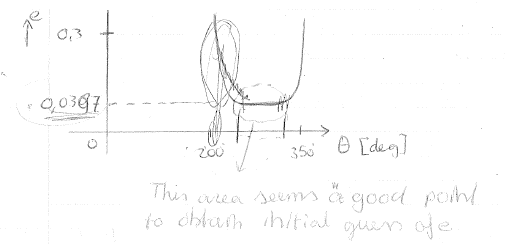
\includegraphics[width=0.6\columnwidth]{Figures/3b.png}
    \caption{First estimate for $\theta$}
    \label{fig:theta}
\end{figure}


\subsection{3c}
\textit{Calculate the values of altitude $h$ of the satellite at $t_0$ and the height of apogee ($h_a$) and perigee ($h_p$) of the orbit} \\

General approach:
For a known $e$ and $\theta$, calculate h using:
\begin{equation}
    h = r-R_E = \frac{p}{1+e \cos(\theta)}-R_E
\end{equation}
As we saw earlier, for the perigee we have:
\begin{equation}
    r_p = \frac{p}{1+e}
\end{equation}

First, find the flight angle using:
\begin{equation}
    \gamma =\arctan \left( \dfrac {\dot{r}}{r\dot{\theta} }\right)
\end{equation}
Then find $V$ using:
\begin{equation}
    V =\dfrac {\dot{r}}{\sin \left( \gamma \right) }
\end{equation}
Then $a$ can be found using:
\begin{equation}
    a=\dfrac {1}{2}\mu \left[ \dfrac {\mu }{r}-\dfrac {1}{2}V^{2}\right] ^{-1}
\end{equation}
Find $p$:
\begin{equation}
    p = a(1-e^2)
\end{equation}
So then the perigee altitude can be found from:
\begin{equation}
    h_p = r_p-R_E = \frac{p}{1+e \cos(\theta)}-R_E
\end{equation}

Since $p$ is the same for the whole orbit, we can then also find the apogee altitude from:
\begin{equation}
    h_a = r_a-R_E = \frac{p}{1-e \cos(\theta)}-R_E
\end{equation}

\subsection{3d}
\textit{Calculate the value of the time interval $t_0 - \tau$, where $\tau$ is the time of last perigee passage. You may use the transformation relation:} 
\begin{equation}
    \tan \left( \dfrac {\theta }{2}\right) =\sqrt {\dfrac {1+e}{1-e}}\tan \left( \dfrac {E}{2}\right) 
\end{equation}
\textit{Further given: $\mu = 398600.4 \, km^3/s^2$, $R=6378.14 \, km$.} \\

For a given $e$ and $\theta$, we can rewrite the given equation to express $E$:
\begin{equation}
    E=2\cdot \arctan \left[ \sqrt {\dfrac {1-e}{1+e}}\cdot \tan \left( \dfrac {\theta }{2}\right) \right] 
\end{equation}

Then, using Kepler's equation:
\begin{equation}
    E-e\cdot \sin \left( E\right) = M
\end{equation}
But since:
\begin{equation}
    M=n\left( t-\tau \right) =\sqrt {\dfrac {\mu }{a^{3}}}\left( t-\tau \right) 
\end{equation}

So then the interval may be found using:
\begin{equation}
    \left( t_{0}-\tau \right) =\dfrac {E-e\sin \left( E\right) }{\sqrt {\dfrac {\mu }{a^{3}}}}
\end{equation}